\documentclass[10pt]{article}
\usepackage[utf8]{inputenc}
\usepackage[T1]{fontenc}
\usepackage{amsmath}
\usepackage{amsfonts}
\usepackage{amssymb}
\usepackage{mhchem}
\usepackage{stmaryrd}
\usepackage{graphicx}
\usepackage[export]{adjustbox}
\graphicspath{ {./images/} }
\usepackage{bbold}

\title{Qualifying Examination Spring 2006, Section on Partial Differential Equations }


\author{August 19, 2020}
\date{}


\begin{document}
\maketitle
April 5, 2006

(Solve three of the problems.)

\begin{enumerate}
  \item Solve the initial value problem
\end{enumerate}
$$
u_{t}+x u_{x}=u
$$
with $u(x, 0)=x^{2}$. Describe and draw the characteristics.

\begin{enumerate}
  \setcounter{enumi}{2}
  \item Using separation of variables, find the eigenfunctions of the Laplace operator with Dirichlet boundary conditions on the rectangle $[0, \pi] \times[0,2 \pi]$.

  \item Assume $u$ is twice continuously differentiable on $[0,1]^{n} \subset R^{n}$, that $u$ is zero on the boundary of that domain and $|\Delta u| \leq 1$. Use the maximum principle to give an estimate of the size of the function $u$.

  \item What is the proper weak solution (i.e. the solution fulfilling the Lax entropy condition) of the equation

\end{enumerate}
$$
u_{t}+u^{3} \cdot u_{x}=0
$$
for the initial values

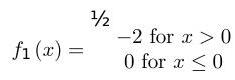
\includegraphics[max width=\textwidth]{2022_05_24_3cb84f0d9d0ada46d202g-01}

and
$$
f_{2}(x)={ }^{1 / 2} \begin{gathered}
0 \text { for } x>0 \\
-2 \text { for } x \leq 0
\end{gathered} ?
$$

\begin{enumerate}
  \setcounter{enumi}{5}
  \item Compute the Fourier series
\end{enumerate}
$$
\sum_{k=0}^{\infty} a_{k} \cos (k x)
$$
for the function

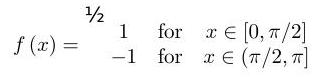
\includegraphics[max width=\textwidth]{2022_05_24_3cb84f0d9d0ada46d202g-01(1)}

on the interval $[0, \pi]$. Also solve the heat equation $u_{t}(x, t)=u_{x x}(x, t)$ on the square $[0, \pi] \times[0, \infty)$ with the initial value $u(x, 0)=f(x)$ and the boundary condition $u_{x}(0, t)=u_{x}(\pi, t)=0$. What does it converge to as $t \rightarrow \infty$ ?

\section{Qualifying Exam: PDE, Fall, 2017}
Choose any three out of the five problems. Please indicate your choice. Show all your work.

\begin{enumerate}
  \item Find the solution to the initial value problem
\end{enumerate}
$$
\begin{aligned}
&u_{t}+\left(\frac{u^{2}}{2}\right)_{x}=0, x \in R, t>0, \\
&u(x, 0)= \begin{cases}2 & x \leq 0 \\
2-x & 0<x \leq 2 . \\
1 & 2<x\end{cases}
\end{aligned}
$$

\begin{enumerate}
  \setcounter{enumi}{2}
  \item Show that if the $C^{1}$ initial data $f(x)$ has $f^{\prime}\left(x_{0}\right)<0$ for some $x_{0}$ and that $F^{\prime \prime}(u) \geq 1$ for all $u$, then the $C^{1}$ solution of
\end{enumerate}
$$
u_{t}+F(u)_{x}=0, \quad u(x, 0)=f(x)
$$
must break down at some time $t>0$. 3. Let $u(x, t)$ and $v(x, t)$ be solutions of the equation $u_{t}-k u_{x x}=q(x, t), \quad x \in R, \quad 0<t \leq T$ satisfy $u(x, 0)=f(x), v(x, 0)=g(x), x \in R$ respectively, where $k>0, T>0$, and $f(x), g(x), q(x, t)$ are continuous and bounded functions. Suppose that $u(x, t)$ and $v(x, t)$ are continuous and bounded on $x \in R, 0 \leq t \leq T$, and that $f(x) \leq g(x), x \in R .$

Show that $u(x, t) \leq v(x, t)$ for $x \in R, 0 \leq t \leq T$. 4. Solve the initial-boundary-value problem
$$
\begin{aligned}
&u_{t}=u_{x x}, \quad 0<x<1, t>0 \\
&u(0, t)=0, \quad u(1, t)=1, \quad t>0 \\
&u(x, 0)=x^{2}, \quad 0<x<1
\end{aligned}
$$
Also find a steady-state solution $U(x)$ of the above problem. 5. Consider the damped wave equation problem

$u_{t t}+d u_{t}-c^{2} u_{x x}=0, \quad x \in R, t>0$,

$u(x, 0)=f(x), \quad u_{t}(x, 0)=g(x), \quad x \in R$

where $c>0, d>0$ and $f, g$ are smooth functions with compact support.

Define energy as $e(t)=\frac{1}{2} \int_{R}\left(u_{t}^{2}(x, t)+c^{2} u_{x}^{2}(x, t)\right) d x$.

Show that the energy is nonincreasing as $t$ increases.

\section{Qualifying Exam: PDE, Spring, 2018}
Choose any three out of the five problems. Please indicate your choice. Show all your work.

\begin{enumerate}
  \item (i) Solve the initial value problem
\end{enumerate}
$$
\begin{aligned}
&u_{t}-\frac{1}{2 x} u_{x}=-u, \quad x>0, t>0, \\
&u(x, 0)=\frac{1}{2+x^{2}}, \quad x \geq 0 .
\end{aligned}
$$
Over what region in the first quarter of the $x$ - $t$ plane does the solution exist? Draw the characteristics on the $x-t$ plane where the solution exists.

(ii) Write an upwind scheme for the above problem. What is the CFL condition for the scheme?

\texttt{https://cdn.mathpix.com/2022_05_24_3cb84f0d9d0ada46d202g-09.jpg}

\begin{enumerate}
  \setcounter{enumi}{2}
  \item Find a weak solution for the nonlinear conservation law with the following Riemann initial data such that the discontinuous solutions satisfy the entropy condition
\end{enumerate}
$u_{t}+(u(1-u))_{x}=0, \quad x \in \mathbb{R}, t>0$

(i) with initial data

$u(x, 0)= \begin{cases}3 & x<0 \\ 2 & x \geq 0\end{cases}$

(ii) with initial data

$u(x, 0)= \begin{cases}2 & x<0 \\ 3 & x \geq 0\end{cases}$ 3. Let $u(x, t)$ and $v(x, t)$ be solutions of the equation $u_{t}-u_{x x}=2, \quad x \in \mathbb{R}, \quad 0<t \leq T$ satisfying $u(x, 0)=f(x), v(x, 0)=g(x), x \in \mathbb{R}$ respectively, where $T>0$, and $f(x), g(x)$ are continuous and bounded functions. Suppose that $u(x, t)$ and $v(x, t)$ are continuous and bounded on $x \in \mathbb{R}$, $0 \leq t \leq T$ and that $f(x) \leq g(x), x \in \mathbb{R} .$

Show that $u(x, t) \leq v(x, t)$ for $x \in \mathbb{R}, 0 \leq t \leq T$. 4. Solve the initial-boundary-value problem

$u_{t}=u_{x x}, \quad 0<x<1, t>0$,

$u(0, t)=1, \quad u(1, t)=3, \quad t>0$,

$u(x, 0)=x, \quad 0<x<1 .$

and also find the steady-state solution $U(x)$ of the above problem. 5. Solve the initial value problem of the wave equation

$u_{t t}-u_{x x}=0, \quad x \in \mathbb{R}, t>0$,

$u(x, 0)=-e^{-x^{2}}, \quad u_{t}(x, 0)=6 x e^{-x^{2}}, \quad x \in \mathbb{R}$.

\section{Qualifying Exam: PDE, Fall, 2019}
Choose any Four out of the five problems. Please indicate your choice. Show all your work.

\begin{enumerate}
  \item Find a weak solution for the nonlinear conservation law with the following Riemann initial data such that the discontinuous solutions satisfy the entropy condition
\end{enumerate}
$u_{t}+(u(2-u))_{x}=0, \quad x \in \mathbb{R}, t>0$,

(i) with initial data
$$
u(x, 0)= \begin{cases}1 & x<0 \\ 2 & x \geq 0\end{cases}
$$
and

(ii) with initial data
$$
u(x, 0)= \begin{cases}2 & x<0 \\ 1 & x \geq 0\end{cases}
$$
\texttt{https://cdn.mathpix.com/2022_05_24_3cb84f0d9d0ada46d202g-15.jpg}

\begin{enumerate}
  \setcounter{enumi}{2}
  \item (i) Solve the initial value problem
\end{enumerate}
$u_{t}-3 x^{2} u_{x}=-u, \quad x \in \mathbb{R}, t>0$,

$u(x, 0)=e^{-2 x^{2}}, \quad x \in \mathbb{R} .$

(ii) Draw the characteristics and find the region in the $x-t$ plane where the solution exists.

(iii) Write an upwind scheme for the above problem.

\texttt{https://cdn.mathpix.com/2022_05_24_3cb84f0d9d0ada46d202g-17.jpg}

\begin{enumerate}
  \setcounter{enumi}{3}
  \item Let both $u(x, t)$ and $v(x, t)$ be solutions of the equation $u_{t}-k u_{x x}=q(x, t), \quad x \in \mathbb{R}, \quad 0<t \leq T$ satisfying $u(x, 0)=f(x)$ and $v(x, 0)=g(x), x \in \mathbb{R}$ respectively, where $k>0, T>0, f(x), g(x)$ and $q(x, t)$ are continuous and bounded on $x \in \mathbb{R}, 0 \leq t \leq T$.
\end{enumerate}
Suppose that $u(x, t)$ and $v(x, t)$ are continuous and bounded on $x \in \mathbb{R}$, $0 \leq t \leq T$, and that $f(x) \leq g(x), x \in \mathbb{R} .$

Show that $u(x, t) \leq v(x, t)$ for $x \in \mathbb{R}, 0 \leq t \leq T$. 4. (i) Solve the initial-boundary-value problem

$u_{t}=u_{x x}, \quad 0<x<1, t>0$,

$u(0, t)=1, \quad u(1, t)=3, \quad t>0$,

$u(x, 0)=x^{2}+x+1, \quad 0 \leq x \leq 1$.

(ii) What is the limit of the solution as $t \rightarrow+\infty$ ? 5. Solve the following initial-boundary-value problem

$u_{t t}-u_{x x}=0, \quad x>0, t>0$,

$u(x, 0)=f(x), \quad u_{t}(x, 0)=g(x), \quad x \geq 0$,

$u_{x}(0, t)=1, \quad t>0$

where $f$ and $g$ are smooth functions satisfying $f^{\prime}(0)=1$ and $g^{\prime}(0)=0$.

\section{Qualifying Exam: PDE, Spring, 2019}
Choose any Four out of the five problems. Please indicate your choice. Show all your work.

\begin{enumerate}
  \item Show that if the $C^{1}$ initial data $f(x)$ has $f^{\prime}\left(x_{0}\right)<0$ for some $x_{0}$, then the $C^{1}$ solution of
\end{enumerate}
$$
u_{t}+\left(u^{2}\right)_{x}=0, \quad x \in \mathbb{R}, t>0, \quad u(x, 0)=f(x)
$$
must break down at some time $t>0$. 2. (i) Solve the initial value problem

$u_{t}+x^{2} u_{x}=-u, \quad x \in \mathbb{R}, t>0$,

$u(x, 0)=x^{2}, \quad x \in \mathbb{R} .$

(ii) Over which region in the $x-t$ plane does the solution exist?

(iii) Write an upwind scheme for the above problem.

\texttt{https://cdn.mathpix.com/2022_05_24_3cb84f0d9d0ada46d202g-23.jpg}

\begin{enumerate}
  \setcounter{enumi}{3}
  \item Solve the following initial boundary value problem
\end{enumerate}
$u_{t}-u_{x x}=0, \quad x>0, t>0$,

$u(x, 0)=f(x), \quad x \geq 0$,

$u(0, t)=1, \quad t \geq 0$

where $f \in C^{2}[0,+\infty)$ is bounded and $f(0)=1$. 4. (i) Solve the initial-boundary-value problem

$u_{t}=u_{x x}, \quad 0<x<1, t>0$,

$u(0, t)=0, u(1, t)=3, \quad t>0$,

$u(x, 0)=x^{2}+2 x, \quad 0 \leq x \leq 1 .$

(ii) What is the limit of the solution as $t \rightarrow+\infty$ ? 5. Consider the damped wave equation problem

$u_{t t}+d u_{t}-c^{2} u_{x x}=0, \quad x \in R, t>0$,

$u(x, 0)=f(x), \quad u_{t}(x, 0)=g(x), \quad x \in R$

where $c>0, d>0$ and $f, g$ are smooth functions with compact support.

Define energy as $e(t)=\frac{1}{2} \int_{R}\left(u_{t}^{2}(x, t)+c^{2} u_{x}^{2}(x, t)\right) d x$.

Show that the energy is nonincreasing as $t$ increases.

\section*{Qualifying Examination on Differential Equations, Fall 2005 }
August 23, 2005

\section{Section on ODE}
(Solve three of the problems)

\begin{enumerate}
  \item Find and classify all equilibria of the system of equations
\end{enumerate}
$$
\begin{aligned}
&x^{\prime}=x+x^{2}+y+y^{2} \\
&y^{\prime}=-x-x^{2}+y+y^{2}
\end{aligned}
$$

\begin{enumerate}
  \setcounter{enumi}{2}
  \item Prove that the system of equations
\end{enumerate}
$$
\begin{aligned}
&x^{\prime}=y+x-x^{3} \\
&y^{\prime}=-x+y-y^{3}
\end{aligned}
$$
has at least one non-constant periodic solution. You may assume that $(0,0)$ is the only equilibrium point.

\begin{enumerate}
  \setcounter{enumi}{3}
  \item Consider the ode $y^{\prime}=f(x)$ with a function $f: \mathbb{R} \rightarrow \mathbb{R}$ which is infinitely differentiable. Estimate the truncation error for one step of the secondorder Taylor method for this equation.

  \item Let $y_{1}$ and $y_{2}$ be two solutions of the equation $x^{\prime}=-x^{2}+t^{2}$, and let $y_{1}(0)=1, y_{2}(0)=2$. Prove that we have $0<y_{1}(t)<y_{2}(t)<y_{1}(t)+1$ for all $t>0$.

\end{enumerate}
\section{Section on PDE}
(Solve three of the problems)

\begin{enumerate}
  \item Compute the Fourier series
\end{enumerate}
$$
\sum_{k=1}^{\infty} a_{k} \sin (k x)
$$
for the function
$$
f(x)=\left\{\begin{array}{lll}
1 & \text { for } & x \in[0, \pi / 2] \\
0 & \text { for } & x \in(\pi / 2, \pi]
\end{array}\right.
$$
on the interval $[0, \pi]$. Also solve the heat equation $u_{t}(x, t)=u_{x x}(x, t)$ on the square $[0, \pi] \times[0, \infty)$ with the initial value $u(x, 0)=f(x)$ and the boundary condition $u(0, t)=u(\pi, t)=0$.

\begin{enumerate}
  \setcounter{enumi}{2}
  \item Using separation of variables, find the eigenfunctions of the Laplace operator with Neumann boundary conditions on the rectangle $[0,1] \times[0,1]$.

  \item Let $B=\left\{x \in \mathbb{R}^{n}|| x \mid<1\right\}$. Show that if $u \in C^{2}(B) \cap C^{0}(\bar{B}), u(x)=0$ for $|x|=1$ and $|\Delta u| \leq K$, then also

\end{enumerate}
$$
-\frac{K}{2 n} \leq u \leq \frac{K}{2 n}
$$
Hint: Use maximum principle for a function $v=u-w$ where $w(x)=0$ for $|x|=1, \Delta w=\pm K$. Note that $w$ is a simple polynomial.

\begin{enumerate}
  \setcounter{enumi}{4}
  \item What is the proper weak solution of the equation
\end{enumerate}
$$
u_{t}+u \cdot u_{x}=0
$$
for the initial values
$$
f_{1}(x)=\left\{\begin{array}{l}
2 \text { for } x>0 \\
0 \text { for } x \leq 0
\end{array}\right.
$$
and
$$
f_{2}(x)=\left\{\begin{array}{l}
0 \text { for } x>0 \\
3 \text { for } x \leq 0
\end{array} ?\right.
$$

\begin{enumerate}
  \setcounter{enumi}{5}
  \item Solve the initial value problem
\end{enumerate}
$$
u_{t}+e^{t} u_{x}=u
$$
with $u(x, 0)=x$. Describe and draw the characteristics $.$

\section*{Qualifying Examination Fall 2006, Section on Partial Differential Equations }
August 23, 2006

(Solve three of the problems.)

\begin{enumerate}
  \item Solve the initial value problem
\end{enumerate}
$$
u_{t}+3 t^{2} u_{x}=u
$$
with $u(x, 0)=x^{2}$. Describe and draw the characteristics.

\begin{enumerate}
  \setcounter{enumi}{2}
  \item Compute the Fourier series
\end{enumerate}
$$
\begin{aligned}
& \sum_{k=0} a_{k} \cos (k x)
\end{aligned}
$$
for the function
$$
\begin{aligned}
& f(x)={ }^{1 / 2} 1 \quad \text { for } \quad x \in[0, \pi / 2]
\end{aligned}
$$
on the interval $[0, \pi]$. Also solve the heat equation $u_{t}(x, t)=u_{x x}(x, t)$ on the square $[0, \pi] \times[0, \infty)$ with the initial value $u(x, 0)=f(x)$ and the boundary condition $u_{x}(0, t)=u_{x}(\pi, t)=0$. What does it converge to as $t \rightarrow \infty$ ?

\begin{enumerate}
  \setcounter{enumi}{3}
  \item What is the proper weak solution (i.e. the solution fulfilling the Lax entropy condition) of the equation
\end{enumerate}
$$
u_{t}+u^{9} \cdot u_{x}=0
$$
for the initial values
$$
f_{1}(x)=\quad \begin{aligned}
&1 / 2 \\
&1 \text { for } x>0 \\
&0 \text { for } x \leq 0
\end{aligned}
$$
and
$$
\begin{gathered}
f_{1}(x)=\quad 0 \text { for } x \leq 0 \\
f_{2}(x)=\quad 1 / 2 \quad 1 \text { for } x>0 \\
-1 \text { for } x \leq 0
\end{gathered} ?
$$

\begin{enumerate}
  \setcounter{enumi}{4}
  \item Assume $u \in C^{2}{ }^{\mathrm{i} \text { (C) }} x \in R^{3}|| x \mid \leq 1^{\underline{a}} \phi, \Delta u \leq 6$ and $u(x) \geq 0$ for $|x|=1$. How small can $u(0)$ become?

  \item Using separation of variables, find the eigenfunctions of the Laplace operator with Neumann boundary conditions on the rectangle $[0,3 \pi] \times[0, \pi]$. Qualifying Exam: PDE, Fall, 2008

\end{enumerate}
Choose any three out of the six problems.

\begin{enumerate}
  \item (i) Solve the initial value problem for the linear equation $u_{t}+\left(x^{2}+1\right) u_{x}=0, x \in R, t>0, u(x, 0)=x^{2}, \quad x \in R$.
\end{enumerate}
(ii) Over what region in the $x$ - $t$ plane does the solution exist? Draw the characteristics on the $x$ - $t$ plane where the solution exists.

\begin{enumerate}
  \setcounter{enumi}{2}
  \item (i) Find the bounded solution $u$ to the following initial-boundary-value problem
\end{enumerate}
$$
\begin{aligned}
&u_{t}-u_{x x}=0, \quad x>0, t>0, \\
&u(x, 0)=f(x), \quad x \geq 0, u(0, t)=2, \quad t \geq 0
\end{aligned}
$$
where $f$ is continuous on $[0,+\infty)$ satisfying $f(0)=2$ and $\sup _{x \geq 0}|f(x)|=$ $M<+\infty$.

(ii) Find the supremum of $|u(x, t)|$ for $x \geq 0$ and $t \geq 0$ in terms of the given data.

\begin{enumerate}
  \setcounter{enumi}{3}
  \item Compute the Fourier series
\end{enumerate}
$$
\Sigma_{k=0}^{+\infty} a_{k} \cos (k x)
$$
for function
$$
f(x)= \begin{cases}1 & x \in\left[0, \frac{\pi}{2}\right] \\ 0 & x \in\left(\frac{\pi}{2}, \pi\right]\end{cases}
$$
on the interval $[0, \pi]$. Also solve the heat equation $u_{t}=u_{x x}$ on $[0, \pi] \times[0,+\infty)$ with the initial value $u(x, 0)=f(x)$ and the boundary conditions $u_{x}(0, t)=$ $u_{x}(\pi, t)=0$. What does the solution converge to as $t \rightarrow+\infty$ ?

\begin{enumerate}
  \setcounter{enumi}{4}
  \item Solve the following initial-boundary-value problem
\end{enumerate}
$$
\begin{aligned}
&u_{t t}-u_{x x}=0, \quad x>0, t>0, \\
&u(x, 0)=f(x), \quad u_{t}(x, 0)=g(x), \quad x \geq 0, \\
&u(0, t)=0, \quad t>0
\end{aligned}
$$
where $f$ and $g$ are smooth functions satisfying $f(0)=g(0)=0$. 5. (i) Find a weak solution satisfying the entropy conditions for $u_{t}+\left(\frac{u^{2}}{2}\right)_{x}=0, \quad x \in R, t>0$, with initial data $u(x, 0)= \begin{cases}2 & x<0 \\ 1 & x \geq 0\end{cases}$ and with initial data $u(x, 0)= \begin{cases}1 & x<0 \\ 2 & x \geq 0\end{cases}$

(ii) Write an upwind scheme for the above problems. What is the CFL condition for the scheme?

\begin{enumerate}
  \setcounter{enumi}{6}
  \item Consider the wave equation problem $u_{t t}-c^{2} u_{x x}=q(x, t), \quad x \in R, t>0$, $u(x, 0)=0, \quad u_{t}(x, 0)=0, \quad x \in R$ where $c>0$ and
\end{enumerate}
$$
q(x, t)= \begin{cases}\left(1-x^{2}\right) \sin t & |x| \leq 1 \\ 0 & |x|>1\end{cases}
$$
Show that $u(x, t)=0$ for $|x|>c t+1$.

\section{Qualifying Exam: ODE, Fall, 2008}
Please choose 4 out of the 6 problems.

\begin{enumerate}
  \item In each case, find the value of $r$ at which bifurcations occur, classify types of bifurcations and sketch the bifurcation diagram of fixed points $x^{*}$ vs $r$.
\end{enumerate}
(a) $\frac{d x}{d t}=r+2 x-x^{2}$;

(b) $\frac{d x}{d t}=r x-x^{3}$.

\begin{enumerate}
  \setcounter{enumi}{2}
  \item Consider the flow on a circle given by $\frac{d \theta}{d t}=1+2 r \cos \theta$.
\end{enumerate}
(a) Draw a phase portrait on the circle for different cases of the control parameter $r$.

(b) Find all bifurcation values of $r$ and draw a bifurcation diagram on the $r \theta$-plane.

(c) Compute the oscillation period when the system is an oscillator.

\begin{enumerate}
  \setcounter{enumi}{3}
  \item Consider the nonlinear system $\frac{d x}{d t}=r-x^{2}, \quad \frac{d y}{d t}=x-y$.
\end{enumerate}
Assume that $r>0$.

(a) Find all fixed points and the linearized system at each fixed point.

(b) Find eigenvalues and corresponding eigenvectors for each linearized system.

(c) Classify each fixed point for the linearized system and for the given nonlinear system. Determine their stability.

(d) Sketch a phase portrait of the given nonlinear system.

\begin{enumerate}
  \setcounter{enumi}{4}
  \item Consider the following model of competition between two species, where $x, y \geq 0$. Find the fixed points, investigate their stability, draw the nullclines and sketch phase portraits. Indicate the basins of attraction of any stable fixed points.
\end{enumerate}
$$
\begin{aligned}
\frac{d x}{d t} &=x(3-2 x-y) \\
\frac{d y}{d t} &=y(2-x-y)
\end{aligned}
$$

\begin{enumerate}
  \setcounter{enumi}{5}
  \item Consider the system
\end{enumerate}
$\frac{d^{2} x}{d t^{2}}=x-4 x^{3}$

Find all the equilibrium points and classify them. Find a conserved quantity.

Sketch the phase portrait.

\begin{enumerate}
  \setcounter{enumi}{6}
  \item Show that the system
\end{enumerate}
$$
\begin{aligned}
&\frac{d x}{d t}=x-y-x\left(x^{2}+y^{2}\right) \\
&\frac{d y}{d t}=x+y-y\left(2 x^{2}+y^{2}\right)
\end{aligned}
$$
has a periodic solution.

Hint: Rewrite the system in polar coordinates and then construct a trapping region.

\section{Qualifying Exam: PDE, Fall, 2020}
Choose any Four out of the five problems. Please indicate your choice. Show all your work.

\begin{enumerate}
  \item Find a weak solution for the nonlinear conservation law with the following Riemann initial data such that the discontinuous solutions satisfy the entropy condition
\end{enumerate}
$u_{t}+(u(1+u))_{x}=0, \quad x \in \mathbb{R}, t>0$,

(i) with initial data
$$
u(x, 0)= \begin{cases}1 & x<0 \\ 2 & x \geq 0\end{cases}
$$
and

(ii) with initial data
$$
u(x, 0)= \begin{cases}2 & x<0 \\ 1 & x \geq 0\end{cases}
$$

\begin{enumerate}
  \setcounter{enumi}{2}
  \item (i) Solve the initial value problem
\end{enumerate}
$u_{t}+x^{2} u_{x}=-u, \quad x \in \mathbb{R}, t>0$,

$u(x, 0)=e^{-x^{2}}, \quad x \in \mathbb{R}$.

(ii) Draw the characteristics and find the region in the $x-t$ plane where the solution exists.

(iii) Write an upwind scheme for the above problem.

\begin{enumerate}
  \setcounter{enumi}{3}
  \item Let $u(x, t)$ and $v(x, t)$ be solutions of the heat equation $u_{t}-k u_{x x}=1, \quad x \in \mathbb{R}, \quad 0<t \leq T$
\end{enumerate}
satisfying

$u(x, 0)=f(x)$ and $v(x, 0)=g(x), x \in \mathbb{R}$

respectively, where $k>0, T>0, f(x)$ and $g(x)$ are continuous and bounded on $x \in \mathbb{R}, 0 \leq t \leq T$.

Suppose that $u(x, t)$ and $v(x, t)$ are continuous and bounded on $x \in \mathbb{R}$, $0 \leq t \leq T$, and that

$f(x) \leq g(x), x \in \mathbb{R} .$

Show that $u(x, t) \leq v(x, t)$ for $x \in \mathbb{R}, 0 \leq t \leq T$. 4. (i) Solve the initial boundary value problem

$u_{t}=u_{x x}, \quad 0<x<1, t>0$,

$u(0, t)=2, u(1, t)=3, \quad t>0$,

$u(x, 0)=x^{2}+2, \quad 0 \leq x \leq 1 .$

(ii) What is the limit of the solution as $t \rightarrow+\infty$ ?

\begin{enumerate}
  \setcounter{enumi}{5}
  \item (i) Solve the initial boundary value problem
\end{enumerate}
$u_{t t}-c^{2} u_{x x}=0, \quad x>0, \quad t \in \mathbb{R}$,

$u(x, 0)=f(x), u_{t}(x, 0)=g(x), x \geq 0$,

$u_{x}(0, t)=0, \quad t \in \mathbb{R}$

where $c>0, f \in C^{2}, g \in C^{1}, f^{\prime}(0)=0$ and $g^{\prime}(0)=0$.

(ii) Assuming further that $f, g$ are of compact support, i.e., $f(x)=g(x)=0$ for $|x|>a$, for some $a>0$, show that the energy

$e(t)=\frac{1}{2} \int_{0}^{+\infty}\left(u_{t}^{2}(x, t)+c^{2} u_{x}^{2}(x, t)\right) d x$

is a conserved quantity as $t$ varies. Choose any three out of the six problems.

\section{Solve the initial value problem}
$u_{t}+x u_{x}=0, \quad x \in R, t>0, u(x, 0)=f(x), \quad x \in R$ where $f(x) \in C^{\mathrm{1}}(R)$. Over what region in the $x$ - $t$ plane does the solution exist? Draw the characteristics on the $x-t$ plane where the solution exists.

\begin{enumerate}
  \setcounter{enumi}{2}
  \item Find a weak solution satisfying the entropy conditions for $u_{t}+\left(u^{3}\right)_{x}=0, \quad x \in R, t>0$, with initial data $u(x, 0)= \begin{cases}2 & x<0 \\ 1 & x \geq 0\end{cases}$ and with initial data $u(x, 0)= \begin{cases}1 & x<0 \\ 2 & x \geq 0\end{cases}$
\end{enumerate}
(ii) Write an upwind scheme for the above problem. What is the CFL condition for the scheme?

\section{Solve the following problem}
where $f(0)=2$. Given that $f(x)$ is continuous and $|f(x)| \leq M$ for $x \geq 0$, find the maximum of $|u(x, t)|$ for $x \geq 0$ and $t \geq 0$.

\begin{enumerate}
  \setcounter{enumi}{4}
  \item Compute the Fourier series $\sum_{k=0}^{+\infty} a_{k} \cos (k x)$
\end{enumerate}
for function
$$
f(x)= \begin{cases}2 & x \in\left[0, \frac{\pi}{2}\right] \\ 0 & x \in\left(\frac{\pi}{2}, \pi\right]\end{cases}
$$
on the interval $[0, \pi]$. Also solve the heat equation $u_{t}=u_{x x}$ on $[0, \pi] \times[0,+\infty)$ with the initial value $u(x, 0)=f(x)$ and the boundary conditions $u_{x}(0, t)=$ $u_{x}(\pi, t)=0$. What does the solution converge to as $t \rightarrow+\infty$ ?

\begin{enumerate}
  \setcounter{enumi}{5}
  \item Solve the initial-boundary-value problem for the wave equation on the half-line
\end{enumerate}
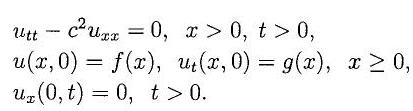
\includegraphics[max width=\textwidth]{2022_05_24_3cb84f0d9d0ada46d202g-37}

\begin{enumerate}
  \setcounter{enumi}{6}
  \item Consider the wave equation with damping $u_{t t}+d u_{t}-c^{2} u_{x x}=0, \quad x \in R, t>0$
\end{enumerate}
$u(x, 0)=f(x), \quad u_{t}(x, 0)=g(x), \quad x \in R$

where $d>0, f$ and $g$ are smooth functions with compact support. Show that the energy $e(t)$ decays as $t$ increases.

\section{Qualifying Exam: PDE, Spring, 2008}
Choose any three out of the six problems.

\begin{enumerate}
  \item (i) Find a weak solution satisfying the entropy conditions for $u_{t}+\left(2 u^{2}\right)_{x}=0, \quad x \in R, t>0$, with initial data $u(x, 0)= \begin{cases}2 & x<0 \\ 1 & x \geq 0\end{cases}$ and with initial data $u(x, 0)=\left\{\begin{array}{ll}1 & x<0 \\ 2 & x \geq 0\end{array}\right.$.
\end{enumerate}
(ii) Write an upwind scheme for the above problem. What is the CFL condition for the scheme?

\begin{enumerate}
  \setcounter{enumi}{2}
  \item (i) Find the bounded solution $u$ to the following initial-boundary-value problem
\end{enumerate}
$$
\begin{aligned}
&u_{t}-u_{x x}=0, \quad x>0, t>0, \\
&u(x, 0)=f(x), \quad x \geq 0, u(0, t)=1, \quad t \geq 0
\end{aligned}
$$
where $f$ is continuous on $[0,+\infty)$ satisfying $f(0)=1$ and $|f(x)| \leq M$ for $x \geq 0$, where $M>0$.

(ii) Find the supremum of $|u(x, t)|$ for $x \geq 0$ and $t \geq 0$ in terms of the given data.

\begin{enumerate}
  \setcounter{enumi}{3}
  \item Compute the Fourier series
\end{enumerate}
$$
\Sigma_{k=1}^{+\infty} b_{k} \sin (k x)
$$
for function
$$
f(x)= \begin{cases}1 & x \in\left[0, \frac{\pi}{2}\right] \\ 0 & x \in\left(\frac{\pi}{2}, \pi\right]\end{cases}
$$
on the interval $[0, \pi]$. Also solve the heat equation $u_{t}=u_{x x}$ on $[0, \pi] \times[0,+\infty)$ with the initial value $u(x, 0)=f(x)$ and the boundary conditions $u(0, t)=$ $u(\pi, t)=0$. What does the solution converge to as $t \rightarrow+\infty$ ?

\begin{enumerate}
  \setcounter{enumi}{4}
  \item Solve the following initial-boundary-value problem
\end{enumerate}
$$
\begin{aligned}
&u_{t t}-u_{x x}=0, \quad x>0, t>0, \\
&u(x, 0)=f(x), \quad u_{t}(x, 0)=g(x), \quad x \geq 0, \\
&u_{x}(0, t)=0, \quad t>0
\end{aligned}
$$
where $f$ and $g$ are smooth functions satisfying $f^{\prime}(0)=0$ and $g^{\prime}(0)=0$. 5. Solve the initial value problem
$$
u_{t}+2 x u_{x}=0, \quad x \in R, t>0, u(x, 0)=f(x), \quad x \in R
$$
where $f(x) \in C^{1}(R)$. Over what region in the $x-t$ plane does the solution exist? Draw the characteristics on the $x-t$ plane where the solution exists.

\begin{enumerate}
  \setcounter{enumi}{6}
  \item Consider the wave equation with damping
\end{enumerate}
$u_{t t}+d u_{t}-c^{2} u_{x x}=0, \quad x \in R, t>0$,

$u(x, 0)=f(x), \quad u_{t}(x, 0)=g(x), \quad x \in R .$

where $c>0, d>0$, and $f, g$ are smooth functions with compact support.

Define the energy $e(t)$ and show that the energy decays as $t$ increases.

\section{Qualifying Exam: PDE, Fall, 2020}
Choose any Four out of the five problems. Please indicate your choice. Show all your work.

\begin{enumerate}
  \item Find a weak solution for the nonlinear conservation law with the following Riemann initial data such that the discontinuous solutions satisfy the entropy condition
\end{enumerate}
$u_{t}+(u(1+u))_{x}=0, \quad x \in \mathbb{R}, t>0$,

(i) with initial data
$$
u(x, 0)= \begin{cases}1 & x<0 \\ 2 & x \geq 0\end{cases}
$$
and

(ii) with initial data
$$
u(x, 0)= \begin{cases}2 & x<0 \\ 1 & x \geq 0\end{cases}
$$

\begin{enumerate}
  \setcounter{enumi}{2}
  \item (i) Solve the initial value problem
\end{enumerate}
$u_{t}+x^{2} u_{x}=-u, \quad x \in \mathbb{R}, t>0$,

$u(x, 0)=e^{-x^{2}}, \quad x \in \mathbb{R}$.

(ii) Draw the characteristics and find the region in the $x-t$ plane where the solution exists.

(iii) Write an upwind scheme for the above problem.

\begin{enumerate}
  \setcounter{enumi}{3}
  \item Let $u(x, t)$ and $v(x, t)$ be solutions of the heat equation $u_{t}-k u_{x x}=1, \quad x \in \mathbb{R}, \quad 0<t \leq T$
\end{enumerate}
satisfying

$u(x, 0)=f(x)$ and $v(x, 0)=g(x), x \in \mathbb{R}$

respectively, where $k>0, T>0, f(x)$ and $g(x)$ are continuous and bounded on $x \in \mathbb{R}, 0 \leq t \leq T$.

Suppose that $u(x, t)$ and $v(x, t)$ are continuous and bounded on $x \in \mathbb{R}$, $0 \leq t \leq T$, and that

$f(x) \leq g(x), x \in \mathbb{R} .$

Show that $u(x, t) \leq v(x, t)$ for $x \in \mathbb{R}, 0 \leq t \leq T$. 4. (i) Solve the initial boundary value problem

$u_{t}=u_{x x}, \quad 0<x<1, t>0$,

$u(0, t)=2, u(1, t)=3, \quad t>0$,

$u(x, 0)=x^{2}+2, \quad 0 \leq x \leq 1 .$

(ii) What is the limit of the solution as $t \rightarrow+\infty$ ?

\begin{enumerate}
  \setcounter{enumi}{5}
  \item (i) Solve the initial boundary value problem
\end{enumerate}
$u_{t t}-c^{2} u_{x x}=0, \quad x>0, \quad t \in \mathbb{R}$,

$u(x, 0)=f(x), u_{t}(x, 0)=g(x), x \geq 0$,

$u_{x}(0, t)=0, \quad t \in \mathbb{R}$

where $c>0, f \in C^{2}, g \in C^{1}, f^{\prime}(0)=0$ and $g^{\prime}(0)=0$.

(ii) Assuming further that $f, g$ are of compact support, i.e., $f(x)=g(x)=0$ for $|x|>a$, for some $a>0$, show that the energy

$e(t)=\frac{1}{2} \int_{0}^{+\infty}\left(u_{t}^{2}(x, t)+c^{2} u_{x}^{2}(x, t)\right) d x$

is a conserved quantity as $t$ varies.

\section{Qualifying Exam: PDE, Fall, 2018}
Choose any Four out of the five problems. Please indicate your choice. Show all your work.

\begin{enumerate}
  \item Show that if the $C^{1}$ initial data $f(x)$ has $f^{\prime}\left(x_{0}\right)>0$ for some $x_{0}$, then the $C^{1}$ solution of
\end{enumerate}
$$
u_{t}+(u(2-u))_{x}=0, \quad x \in \mathbb{R}, t>0, \quad u(x, 0)=f(x)
$$
must break down at some time $t>0$. 2. (i) Solve the initial value problem

$u_{t}-x^{2} u_{x}=-u, \quad x \in \mathbb{R}, t>0$,

$u(x, 0)=f(x), \quad x \in \mathbb{R}$

where $f \in C^{1}(\mathbb{R})$.

(ii) Over which region in the $x-t$ plane does the solution exist?

(iii) Write an upwind scheme for the above problem.

\texttt{https://cdn.mathpix.com/2022_05_24_3cb84f0d9d0ada46d202g-44.jpg}

\begin{enumerate}
  \setcounter{enumi}{3}
  \item Solve the following initial boundary value problem
\end{enumerate}
$u_{t}-k u_{x x}=0, \quad x>0, t>0$,

$u(x, 0)=f(x), \quad x \geq 0$,

$u_{x}(0, t)=1, \quad t \geq 0$.

where $k>0, f \in C^{2}[0,+\infty)$, is bounded and $f^{\prime}(0)=1$. 4. (i) Solve the initial-boundary-value problem

$u_{t}=u_{x x}, \quad 0<x<1, t>0$,

$u(0, t)=1, u(1, t)=2, \quad t>0$,

$u(x, 0)=x^{2}+1, \quad 0 \leq x \leq 1 .$

(ii) What is the limit of the solution as $t \rightarrow+\infty$ ? 5. Solve the initial value problem of the wave equation

$u_{t t}-4 u_{x x}=0, \quad x \in \mathbb{R}, t>0$,

$u(x, 0)=-e^{-x^{2}}, \quad u_{t}(x, 0)=12 x e^{-x^{2}}, \quad x \in \mathbb{R} .$

\section*{Qualifying Exam for Math 5600 }


\section*{Dr. Zahra Aminzare }
\section{INSTRUCTION:}
\begin{itemize}
  \item The questions for this exam (Math 5600) are divided into two parts.
\end{itemize}
Answer both questions in Part I.

\section{Answer only one question in Part II.}
\begin{itemize}
  \item If you work on more than one question in Part II, please state clearly which one should be graded.

  \item No additional credit will be given for more than one of the questions in Part II.

  \item If no choice between the questions is indicated, then the first optional question attempted will be the only one graded.

  \item All the questions have equal points.

  \item Please start a new page for every new question and put your name on each sheet.

  \item Please turn in the exam questions with your solutions.

  \item Please turn in the scratch papers. All scratch papers will be discarded.

\end{itemize}
\section{Good Luck!}
\section{Part I. Please answer $\underline{\text { BOTH }}$ questions 1 and $2 .$}
Question 1. Consider the motion of an undamped harmonic oscillator, given by the equation
$$
\ddot{x}=-4 x,
$$
where $x(t)$ represents the location of the oscillator, and $\ddot{x}$ denotes the second derivative of $x$ with respect to $t$.

(a) Introduce a new variable $y$ for the velocity of the oscillator and formulate the motion of the harmonic oscillator as a two dimensional linear system of the form $\dot{X}=A X$, where $X=(x, y)^{\top}$ and $A$ is a $2 \times 2$ matrix.

(b) Find the eigenvalues and eigenvectors of $A$.

(c) Show there exists an invertible matrix $T$ so that $T^{-1} A T=B$ where $B$ is in Jordan canonical form.

(d) Use the Jordan canonical form to find the general solution of the system $\dot{X}=A X$.

Question 2. Consider the system
$$
\begin{aligned}
\dot{x} &=y-a x \\
\dot{y} &=-a y+\frac{x}{1+x},
\end{aligned}
$$
where $a$ is a positive parameter. Answer the following questions.

(a) For each qualitatively different value of $a>0$, find all equilibrium points. When the Hartman-Grobman theorem applies, classify each equilibrium point.

(b) Describe the bifurcation that occurs as $a$ varies and find the critical value of $a$ (call it $a^{*}$ ) at which the bifurcation occurs. (You do not need to compute the center manifold at $a=a^{*}$.)

(c) Sketch the phase plane (phase portrait) for $a>a^{*}$ which qualitatively describes the full dynamics of the system. Hint: You should indicate the equilibrium points, a heteroclitic orbit, the stable and unstable curves, and six trajectories.

\section{Part II. Please answer ONLY ONE of the following questions.}
Question 3. Consider
$$
\begin{aligned}
\dot{x} &=y-x \\
\dot{y} &=x-y-x z \\
\dot{z} &=x y-z .
\end{aligned}
$$
(a) State the definitions of a (Lyapunov) stable equilibrium point and an asymptotically stable equilibrium point.

(b) Is the origin $(0,0,0)^{\top}$ a (Lyapunov) stable equilibrium point or asymptotically stable equilibrium point?

(c) What is the basin of attraction?

Hint: Find an appropriate Lyapunov function and use LaSalle's invariance principle.

Question 4. Consider the system
$$
\begin{aligned}
\dot{x} &=x(1-r)-y \\
\dot{y} &=y(1-r)+x,
\end{aligned}
$$
where $r^{2}=x^{2}+y^{2}$. This system has a periodic solution $\gamma(t)=(\cos (t), \sin (t))^{\top}$. Determine the stability of $\gamma(t)$.

Hint: You may use ONE (and only one) of the following methods:

\begin{enumerate}
  \item Compute the characteristic multipliers for $\gamma(t)$. (Liouville's Formula may help.)

  \item Compute the Poincaré map of $\gamma(t)$. (Polar coordinate transformation may help.)

\end{enumerate}

\end{document}